\documentclass{endm}
\usepackage{endmmacro}
\usepackage{graphicx}

% The following is enclosed to allow easy detection of differences in
% ascii coding.
% Upper-case    A B C D E F G H I J K L M N O P Q R S T U V W X Y Z
% Lower-case    a b c d e f g h i j k l m n o p q r s t u v w x y z
% Digits        0 1 2 3 4 5 6 7 8 9
% Exclamation   !           Double quote "          Hash (number) #
% Dollar        $           Percent      %          Ampersand     &
% Acute accent  '           Left paren   (          Right paren   )
% Asterisk      *           Plus         +          Comma         ,
% Minus         -           Point        .          Solidus       /
% Colon         :           Semicolon    ;          Less than     <
% Equals        =           Greater than >          Question mark ?
% At            @           Left bracket [          Backslash     \
% Right bracket ]           Circumflex   ^          Underscore    _
% Grave accent  `           Left brace   {          Vertical bar  |
% Right brace   }           Tilde        ~

\newcommand{\Nat}{{\mathbb N}}
\newcommand{\Real}{{\mathbb R}}
\def\lastname{Please list your Lastname here}

\begin{document}

% DO NOT REMOVE: Creates space for Elsevier logo, ScienceDirect logo
% and ENDM logo
\begin{verbatim}\end{verbatim}\vspace{2.5cm}

\begin{frontmatter}

\title{Hoy te convert\'is en (Junior) Data Scientist}

\author{Cort\'es Lucas \thanksref{lucasemail}, Lamela Emanuel \thanksref{emanuelemail}, Zimenspitz Ezequiel \thanksref{ezequielemail}}
\address{Universidad de Buenos Aires\\ Buenos Aires, Argentina}

\thanks[lucasemail]{lucascortes@me.com, LU: 302/13}
\thanks[emanuelemail]{emanuel93\_13@hotmail.com, LU: 021/13}
\thanks[ezequielemail]{ezeqzim@gmail.com, LU: 155/13}

\begin{abstract}

En este trabajo analizamos la tem\'atica de los desv\'ios en los vuelos en realaci\'on a principalmente 2 ejes: la \'epoca del a\~no y la distancia del trayecto. 

En el caso de la \'epoca del a\~no, se puede observar que para distintos Estados de USA la curva de desv\'ios tiene picos en distintas \'epocas del a\~no, mientras que para el caso de la distancia del trayecto se observa que al aumentar esta, existe un aumento paulatino de desv\'ios. Por otro lado, encontramos que existen ciertos trayectos con picos exponenciales de desv\'ios.

Por \'ultimo creamos modelos predictivos para cada una de nuestras m\'etricas utilizando cuadrados m\'inimos lineales y creando familias de funciones adecuadas a cada modelo particular.

\end{abstract}

\begin{keyword}
Modelos predictivos, Data fitting, Cuadrados m\'inimos lineales, Desv\'ios a\'ereos
\end{keyword}

\end{frontmatter}

"¿Qu\'e equipo/qui\'en crees que gana hoy?", una simple pregunta que es dif\'icil de responder con certeza dada la cantidad de aspectos que ofrecen los deportes en general. Antes de analizar una manera de responder la misma con datos y fundamentos te\'oricos, abocamos en algunos casos en los cuáles esto ser\'ia \'util:

\begin{itemize}
\item \textbf{Inversiones:} Convencer de que fortalecer financieramente a una entidad/un jugador es seguro.
\item \textbf{Puntuaci\'on:} En determinados deportes o contextos, vencer a distintos oponentes no siempre genera la misma cantidad de puntos. Esto ayuda a determinar una valuaci\'on de los mismos.
\item \textbf{Medici\'on:} Podr\'ia aportar m\'etricas internas para determinar c\'omo se encuentra la entidad/el jugador comparativamente con los dem\'as.
\end{itemize}

Proveer metodolog\'ias que incorporen aspectos varios y relevantes de los encuentros es esencial para que incremente su precisión. Dicho esto, el m\'etodo que utilizaremos es el \textbf{\textit{Colley Matrix Method}} \textbf{[1]}.

\subsection{Colley Matrix Method}

Este m\'etodo busca obtener las probabilidades de que cada equipo de una liga gane su pr\'oximo encuentro, teniendo en consideraci\'on el schedule que atraves\'o cada uno de ellos (jugar contra los mejores equipos al inicio no indica que vaya a perder contra los peores en los subsiguietntes partidos), sin importar la diferencia de la cantidad de partidos jugados por cada equipo y solo considerando si el equipo gan\'o o perdi\'o (no la diferencia en puntajes obtenidos en los mismos). Es necesario notar que s\'olo aplica a modelos de competencias que no admiten empate como un resultado posible, como los que analizaremos en este contexto.

Definamos primero el modelo utilizado para el problema. Sea $\Gamma = \{1,2,...,T\}$ el conjunto de participantes de la competencia. Luego, para cada equipo \bm{$i \in \Gamma$} denominamos \bm{$n{_i}$} all n\'umero total de partidos jugados por el equipo $i$, \bm{$w{_i}$} al n\'umero de partidos ganados por el equipo $i$ y, an\'alogamente, \bm{$l{_i}$} a la cantidad de encuentros por el equipo $i$. Por \'ultimo, dados $i, j \in \Gamma$, $i \neq j$, \bm{$n{_i}{_j}$} al n\'umero de enfrentamientos entre $i$ y $j$. Una vez definido esto, a través de una serie de postulados y argumentos matemáticos, el paper \textbf{[1]} plantea que las probabilidades se obtienen como resultado de un sistema de ecuaciones lineales de la forma \bm{$Cr = b$}. \\

Donde:

\begin{itemize}
\item 
$C \in R^{T \times T}, C{_i}{_j} =
\left\{
	\begin{array}{lcc}
		-n{_i}{_j} & si & i \neq j \\
		\\ 2 + n{_i} & si & i = j \\
	\end{array}
\right.$
\item $r \in R^{T}$, donde $r{_i} = $ probabilidad de que el equipo i gane su siguiente partido
\item $b \in R^{T}$, donde $b{_i} = 1 + (w{_i} - l{_i}) / 2$
\end{itemize}

Por lo tanto, lo que se busca despejar son los elementos del vector $r$.

$C$ se denomina la \textbf{matriz de Colley} que particularmente, por lo demostrado en \textbf{[1]}, es \textbf{sim\'etrica} ($A = A{^t}$) y \textbf{definida positiva} (\textcolor{red}{DEFINITION HERE}).

Para resolver este sistema, usaremos dos algoritmos distintos para obtener sistemas de f\'acil resoluci\'on por \textit{back-substitution} y \textit{forward-substitution}. \textit{Eliminaci\'on Gaussiana} y \textit{Factorizaci\'on de Cholesky}.

\subsubsection{Eliminaci\'on Gaussiana}

La eliminaci\'on gaussiana es un algoritmo que transforma un sistema de ecuaciones en un sistema equivalente, con la caracter\'istica de que este nuevo sistema es triangular superior.

Esto se logra a través de operaciones que no alteran el conjunto solución de un sistema:

\begin{itemize}
\item Multiplicar una ecuación por un escalar
\item Intercambiar ecuaciones
\item Sumar a una ecuación con un múltiplo de otra
\end{itemize} 

Luego se resuelve por back-substitution y obtenemos el resultado deseado. Sea $A \in R^{nxn}, n \in N$. El sistema $Ax = b$ se transforma en uno equivalente $Ux = b'$, con $U$ una matriz triangular superior. \\

Los $x{_i}$ se obtienen de la siguiente manera: \\

$x{_i} = (b'{_i} - \sum\limits_{j = i + 1}^n u_{ij}x_{i}) / u_{ii}$ \\

Se puede observar que si $\exists \, i \in \{1, ..., n\} / a_{ii} = 0$ entonces no se puede realizar este procedimiento. De todas formas, en este trabajo podemos asegurar que la eliminaci\'on encuentra la $U$ y m\'as a\'un, el sistema tiene soluci\'on \'unica porque la matriz de Colley es, como se mencion\'o anteriormente, sim\'etrica y definida positiva.

Dentro del contexto de uso del \textbf{CMM}, utilizamos la Eliminaci\'on Gaussiana para obtener los $r_i$.

\subsubsection{Factorizacio\'on de Cholesky}

La factorizaci\'on de Cholesky es un caso particular de una factorizaci\'on LU, con L matriz triangular inferior y U matriz triangular superior. Bajo la hip\'otesis de este trabajo sobre las caracter\'isticas de la matriz de Colley, podemos afirmar que existe una factorizaci\'on de la forma LU de C, tal que $U = L{^t}$. \\

$LL{^t}{_i}{_j} =
\left\{
	\begin{array}{lcc}
		\sqrt{C{_i}{_i} - \sum\limits_{k=1}^{i-1} L{_i}{_k}^2} & si & i = j \\
		\\ \frac{1}{L{_i}{_i}}(C{_i}{_j} - \sum\limits_{k=1}^{i-1} L{_i}{_k}L{^t}{_j}{_k}) & si & i \neq j \\
	\end{array}
\right.$ \\

Luego, el sistema equivalente ser\'a $LL{^t}x = b$, entonces puedo resolver $Ly = b$ por forward-substitution y luego $L{^t}x = y$ para obtener el resultado deseado por back-substitution.

\textcolor{red}{\textbf{TODO: Escribir, no olvidar de mencionar por qu\'e y para que se utiliza.}}

El suelo est\'a labrado en cuestiones te\'oricas. En esta secci\'on nos avocaremos en explicar el papel que juega cada m\'etodo y, el proceso completo partiendo de las im\'agenes y concluyendo en su clasificaci\'on.

Vamos a considerar las im\'agenes, siendo $n \in \mathbb{N}$ la cantidad, como $x^{(i)} \in \mathbb{R}^{m}$ con $m = 28 \times 28 = 784$ y $i \in \{1, ..., n\}$. Al conjunto de im\'agenes lo denominamos $I$. Como est\'an en escala de grises, adem\'as se cumple que $x^{(i)}_{j} \in \{0, ..., 255\}$, d\'onde $x^{(i)}_{j}$ es el $j$-esimo elemento de $x_{i}$, $\forall j \in \{1, ..., 784\}$. En t\'erminos coloquiales, una \textit{tira} de 784 valores que est\'an en el rango de 0 a 255. Adicionalmente, el conjunto $C = \{0, ..., 9\}$ es el conjunto de clases/\textit{labels}/\textit{tags}/d\'igitos, seg\'un como los denominemos en cada ocasi\'on particular. Finalmente, por ahora, vamos a considerar una partici\'on de $I = A \cup B$, d\'onde $A$ e $B$ son dijuntos y los mismos tienen las particularidades destacadas en \ref{intro_consideraciones}.

\subsection{Metodolog\'ias de Clasificaci\'on}

\subsubsection{Clasificaci\'on \textit{naive} con kNN}

En una primera aproximaci\'on, \textbf{utilizamos el kNN como m\'etodo de clasificaci\'on a secas}, lo que es decidir a qu\'e d\'igito pertenece cada imagen del conjunto $A$. Tomamos $a \in A$ una tira que buscamos \textit{taggear}.

Recordar que, por c\'omo lo definimos en la \textit{secci\'on \ref{intro_knn}}, el algoritmo requer\'ia \textbf{una funci\'on de distancia $\mathbf{d}$}. Como modelamos con vectores, proponemos la \textbf{\textit{norma 2}}. En otras palabras, siendo $z$ y $x$ dos im\'agenes $d(z,x) = \vert\vert z - x \vert\vert_2^2 = (z - x)^{t}(z - x)$. Notar que en su forma de \textit{producto interno}, el c\'omputo no pierde precisi\'on por ser suma y multiplicaci\'on de n\'umeros entre $0$ y $255$. Adicionalmente, fue elegida por el nivel de precisi\'on que posee (en definitiva, compara una a una cada componente). 

En consecuencia de haber definido una $d$, \textbf{obtenemos el conjunto de \textit{$\mathbf{k}$ vecinos m\'as cercanos}}. Clasificar es f\'acil: se cuentan las etiquetas de cada uno de los $k$ vecinos y la que m\'as se repita, se le asigna a $a$ \footnote{En caso de empate, nos quedamos con el primero que hayamos encontrado que maximice la cantidad de apariciones}.

Desafortunadamente, \textbf{la simplicidad tiene su costo temporal en este caso}. Las im\'agenes tienen $784$ pixels, es decir, cada punto a considerar tiene $784$ componentes. Calcular la distancia de un punto de esta dimensi\'on contra \textit{$\vert B \vert$} (el tamaño de $B$) de la misma dimensi\'on suena a mucho trabajo y \textit{lo es}. Aqu\'i es d\'onde cobran valor \textbf{PCA} y \textbf{PLS-DA}.

Ambos tienen la misma idea, obtener una matriz que realice un cambio de base tal que permita quedarnos con s\'olo una \textit{porci\'on}, la de mayor contenido de informaci\'on, de la misma. Aunque por s\'i solos, no son m\'etodos de categorizaci\'on. Por ende, \textbf{estar\'an involucrados como \textit{preprocesadores} de la informaci\'on a ser servida al \textit{kNN}} (reducir las dimensiones a considerar previo a aplicar \textit{kNN}).

\subsubsection{Reducci\'on de dimensi\'on \textit{no} supervisada con \textit{PCA}}

Siguiendo la l\'inea de \textbf{PCA} (\ref{intro_PCA}), buscamos $P$ conformado por las \textit{\textbf{Componentes Principales}} que son los autovectores de $M_{X}$. Inmediatamente surge una imposici\'on en costo de c\'omputo muy elevada: Dado que $M_{X} \in \mathbb{R}^{784 \times 784}$ es sim\'etrica, posee \textit{rango completo} de autovectores. Calcular los $784$ autovectores es pesado, y ,a\'un provisto de ellos, multiplicar \textit{todas} las im\'agenes contra la matriz generada tambi\'en lo es. Esto es bloqueante, lo que busc\'abamos era \textit{reducir} el problema en dimensi\'on para alivianar el costo de c\'omputo.

Provisto de $\alpha \in \mathbb{N}$, y $n_{iter} \in \mathbb{N}$, buscamos generar la transformaci\'on $P \in R^{\alpha \times 784}$ tal que contenga $\alpha$ \textbf{\textit{Componentes Principales}} como filas.
Como dichas componentes son los autovectores, buscamos $\alpha$ autovalores y autovectores de la matriz de covarianzas $M_{X}$. Pero al tomar un n\'umero menor de componentes, se pierde informaci\'on. Por eso mismo, decidimos \textbf{buscar las que maximicen la varianza}, son las que m\'as informaci\'on poseen en el espacio de informaci\'on transformado. Recordando el fundamento del m\'etodo planteado en la secci\'on anterior, buscabamos los autovectores de $M_{X}$ dado que la diagonalizaban. Al estar diagonalizada, los autovalores son los elementos de la diagonal, que a su vez son las varianzas de las variables en \textit{nuevo espacio de datos}. Obtener los de mayor m\'odulo nos aporta la mayor cantidad de informaci\'on posible. Para esto aplica el \textbf{M\'etodo de la Potencia} (explicado en \ref{desarrollo_metodo-potencia}), iterando tantas veces como el $n_{iter}$ provisto, combinado con \textbf{Deflaci\'on} (desarrollado en \ref{desarrollo_deflacion}). Repetimos $\alpha$ veces un paso $i$, con $B^0 = M_{X}$, de: obtener $\lambda_{i}$, el $i$-\'esimo autovalor ordenas por m\'odulo, asociado a $v_{i}$, calcular $B^{i + 1} = B^{i} - \lambda_{i}v_{i}v_{i}^{t}$ y comenzar el paso $i+1$.

Antes de continuar, los algoritmos de generaci\'on de autovectores tienen condiciones sobre los cu\'ales funcionan.

Para el caso de m\'etodo de la potencia:

\begin{itemize}
\item \textcolor{red}{// TODO: Agregar}
\item Como $M_{X}$ es sim\'etrica, tiene todos los autovalores reales.
\end{itemize}

Los requerimientos de deflaci\'on se cumplen dado que:

\begin{itemize}
\item Al ser $M_{X}$ sim\'etrica, sus autovectores generan una \textbf{base ortonormal}.
\end{itemize}

Con lo cu\'al nos quedamos con una matriz $P$ que posee, por filas, los $\alpha$ autovectores de $M_{X}$ que mayor informaci\'on almacenan. El siguiente paso es aplicar el \textit{cambio de base} a cada muestra $z \in Z$ y a $y$: $Py = \hat{y} \in \mathbb{R}^{\alpha}$ y $\hat{z} = Pz \in \mathbb{R}^{\alpha}$, obteniendo sus correspondientes \textit{\textbf{Transformaciones Caracter\'isticas}}. A dicha transformaci\'on la denominamos $\mathbf{tc_{PCA}}$.

\subsubsection{Reducci\'on de dimensi\'on supervisada con \textit{PLS-DA}} \label{desarrollo_PLSDA}

Presentamos un \textit{pseudo-c\'odigo} del procedimiento para luego explicar las decisiones involucradas y las condiciones correspondientes que se deben dar para su correctitud: \\

\begin{algorithm}
\begin{algorithmic}[1]
\FOR {$i \leftarrow [1..\gamma]$}
\STATE {$M_{i} \leftarrow X^{t}YY^{t}X$}
\STATE {$w_{i} \leftarrow$ autovector asociado al mayor autovalor de $M_{i}$} \COMMENT {Deber\'ia estar normalizado, si no, normalizar}
\STATE {$t_{i} \leftarrow Xw_{i}$}
\STATE {Normalizar $t_{i}$}
\STATE {$X \leftarrow X - t_{i}t_{i}^{t}X$}
\STATE {$Y \leftarrow Y - t_{i}t_{i}^{t}Y$}
\ENDFOR
\RETURN {$w_{i}$ para cada $i \leftarrow [1..\gamma]$}
\end{algorithmic}
\caption{PLS($X, Y, \gamma$)}
\end{algorithm}

El algoritmo recibe $X \in R^{n \times 784}$, la matriz de imagenes centralizadas por la media, e $Y$ un vector que \textit{mapea} cada posici\'on con la etiqueta de la im\'agen que se encuentra en la susodicha posici\'on en $X$. Dadas estas construcciones, buscamos ir obteniendo iterativamente los \textbf{autovectores dominantes} $w_{i}$ (autovectores cuyos autovalores sean dominantes en el paso $i$) sobre la matriz $M_{i}$. Notemos que $M_{i}$ es sim\'etrica en todos los pasos: siendo $X = X_{i}$, $Y = Y_{i}$ las matrices iniciales en el paso $i$, vemos que $M_{i}^{t} = (X^{t}YY^{t}X)^{t} = (Y^{t}X)^{t}(X^{t}Y)^{t} = X^{t}(Y^{t})^{t}Y^{t}(X^{t})^{t} = X^{t}YY^{t}X = M_{i}$. Como, por lo desarrollado en \ref{intro_PLSDA}, requerimos $w_{i}$ autovector dominante, utilizamos el \textbf{M\'etodo de la Potencia} (\ref{desarrollo_metodo-potencia}) para extraerlo. El vector resultado se encuentra normalizado, por ende podemos evitar el paso de normalizaci\'on siguiente a su obtenci\'on. Para finalizar la iteraci\'on, en base a $w_{i}$, $X_{i}$ e $Y_{i}$, calcular $t_{i}$ como $Xw_{i}$ para realizar el c\'omputo de $X_{i+1}$ e $Y_{i+1}$.

Las $\gamma$ repeticiones de estos calculos nos otorga $w_{1}$, ..., $w_{\gamma}$ y los utilizamos para obtener la \textbf{Transformaci\'on Caracter\'istica} de una im\'agen $x_{i}$ como $\mathbf{tc_{PLS}(x_{i})} = (w_{1}^{t}x_{i}, ..., w_{\gamma}x_{i}) \in R_{\gamma}$.

\textbf{Con este planteo, tenemos un PLS tracicional}. \textbf{La extensi\'on a PLS-DA la hacemos tomando la $\mathbf{Y}$ como una matriz que centraliza}, como a $X$, \textbf{a una matriz que tiene un $1$ en la posici\'on $(i, j)$ si la imagen $i$ tiene etiqueta $j$\footnote{Indexando desde 1} o $(-1)$ en caso contrario}.

\subsubsection{Clasificaci\'on inteligente: \textit{Transformaci\'on} + \textit{kNN}}

Tanto \textit{PCA} como \textit{PLS-DA} nos facilitan una \textit{transformaci\'on caracter\'istica} que reduce la dimensi\'on de las im\'agenes. Pero \textbf{por s\'i mismos no son \textit{clasificadores}}. Que la dimensi\'on de las im\'agenes se encuentre reducida, abre la posibilidad de utilizar el \textit{kNN} y que su ejecuci\'on se complete en tiempos razonables.

Por lo tanto, \textbf{el algoritmo completo de clasificaci\'on}, sobre una im\'agen particular $y \in Y$ a clasificar, se compone de tomar una $\mathbf{tc_{m}}$, la transformaci\'on caracter\'istica de \textit{PCA} o \textit{PLS-DA}, obtener $tc_{m}(y)$ y $tc_{m}(z_{i})$, con $z_{i} \in Z$, y finalmente utilizar el criterio de clasificaci\'on provisto por \textit{kNN}.

\subsection{Estrategias de medici\'on}

\subsubsection{Evaluaci\'on robusta con \textit{K-fold cross validation}}

\textcolor{red}{// TODO: Fill}

\subsubsection{M\'etricas de calidad}

Finalmente, se desarrollaron algunas m\'etricas para medir qu\'e tan buenas son las decisiones tomadas por el clasificador: \\

* \underline{\textbf{Precision:}} Es una \textbf{medida de cu\'antos aciertos relativos tiene un clasificador dentro de una clase particular}. Es decir, dada una clase $i$, la precision de dicha clase es $tp_{i} / (tp_{i} + fp_{i})$.

En la anterior f\'ormula, $tp_{i}$ son los \textit{verdaderos positivos} de la clase $i$. Es decir, muestras que realmente pertenec\'ian a la clase $i$ y fueron exitosamente identificadas como tales. En contraposici\'on, $fp_{i}$ son los \textit{falsos positivos} de la clase $i$. Son aquellas muestras que fueron identificadas como pertenecientes a la clase $i$ cuando realmente no lo eran.

Luego, la \textit{precision} en el caso de un clasificador de muchas clases, se define como \textbf{el promedio de las precision para cada una de las clases}. \\

* \underline{\textbf{Recall:}} Es una \textbf{medida de que tan bueno es un clasificador para, dada una clase particular, identificar correctamente a los pertenecientes a esa clase}. Dada una clase $i$, el recall de dicha clase es $tp_{i} / (tp_{i} + fn_{i})$.

En la anterior f\'ormula, $fn_{i}$ son los \textit{falsos negativos} de la clase $i$. Es decir, muestras que pertenec\'ian a la clase $i$ pero que fueron identificadas con otra clase.

Luego, el \textit{recall} en el caso de un clasificador de muchas clases, se define como \textbf{el promedio del recall para cada una de las clases}. \\

* \underline{\textbf{F1-Score:}} Dado que precision y recall son dos medidas importantes que no necesariamente tienen la misma calidad para un mismo clasificador, se define esta m\'etrica para \textbf{medir un compromiso entre ambas}. Se define como $2 * precision * recall / (precision + recall)$.

\subsection{Algoritmos de Utilidad}

\subsubsection{M\'etodo de la Potencia}\label{desarrollo_metodo-potencia}

Tenemos una necesidad de encontrar \textit{autovalores} con sus \textit{autovectores asociados}. Para esto utilizamos el \textbf{M\'etodo de la Potencia}. Sea $B^{n \times n}$ la matriz de entrada.

\begin{algorithm}
\begin{algorithmic}[1]
\STATE {$v \leftarrow x_{0}$}
\WHILE {No se cumpla la condici\'on de finalizaci\'on}
\STATE {$v \leftarrow Bv$}
\STATE {Normalizar $v$}
\ENDWHILE
\STATE {$\lambda \leftarrow v^{t}Bv$}
\RETURN {$\lambda, v$}
\end{algorithmic}
\caption{M\'etodo de la Potencia($B, x_{0}$, condici\'on de finalizaci\'on)}
\end{algorithm}

Este m\'etodo busca un autovector $v_{1} \in \mathbb{R}^{m}$ tal que $\vert\vert v \vert\vert_{2} = 1$ aproximando el pasado como par\'ametro iterativamente, con la particularidad de que se corresponde con el autovalor $\lambda_{1} \in \mathbb{R}$ de manera que $\lambda_{1} > \lambda_{i}$ autovalor con $i \neq 1$. Una condici\'on para que converja a este vector es \textcolor{red}{TODO}, notar que para dimensiones grandes, la probabilidad de elegir un vector inicial al azar es pr\'acticamente nula, de modo que el $x_{0}$ es elegido en forma aleatoria. La otra condici\'on es que $B$ tenga todos los autovalores reales. Veremos como ambas condiciones se cumplen para las matrices a las cu\'ales son aplicadas.

\subsubsection{Deflaci\'on}\label{desarrollo_deflacion}

Este algoritmo soslayar\'a un esquema iterativo en el cu\'al uno puede obtener autovalores y autovectores.

Sea $B \in R^{n \times n}$ una matriz que posee autovalores distintos $\lambda_{1}, ..., \lambda_{n}$ con autovectores $v_{1}, ..., v_{n}$ asociados tales que $\vert \lambda_{1} \vert > ... > \vert \lambda_{n} \vert$, en otras palabras poder ordenarlos por m\'odulo. Adem\'as se pide que los autovectores generen una base ortonormal. \textcolor{red}{// TODO: Ver por qu\'e no hace falta que los autovalores no sean distinos} Veamos entonces que: \\

$(B - \lambda_{1}v_{1}v_{1}^{t})v_{1} = Bv_{1} - \lambda_{1}v_{1}(v_{1}^{t}v_{1}) = \lambda_{1}v_{1} - \lambda_{1}v_{1} = 0v_{1}$

$(B - \lambda_{1}v_{1}v_{1}^{t})v_{i} = Bv_{i} - \lambda_{1}v_{1}(v_{1}^{t}v_{i}) = \lambda_{i}v_{i}$ \\

Por lo tanto, la matriz $B - \lambda_{1}v_{1}v_{1}^{t}$ posee autovalores $0, \lambda_{2}, ..., \lambda_{n}$ asociados a $v_{1}, ..., v_{n}$ de tal forma que puedo repetir el proceso obteniendo $\lambda_{2}$ y $v_{2}$. Este algoritmo se acopla muy bien con el M\'etodo de la potencia puesto que el susodicho extrae el autovalor dominante y su correspondiente autovector, con lo cu\'al es perfecto para una combinaci\'on de ambos.

\section{Experimentos y Discusi\'on}
\subsection{Desv\'ios}

En este experimento realizamos un an\'alisis sobre los desv\'ios de los vuelos en base al tiempo. Dividimos al año en 12 meses y tomamos el per\'iodo 2000-2008. Para generar un an\'alisis representativo del comportamiento a escala pa\'is decidimos tomar 2 estados con caracter\'isticas particulares: deben tener gran cantidad de vuelos de llegada y deb\'ia ser uno de cada costa. De este modo tomamos a los estados de California y Florida para realizar el an\'alisis.

\subsubsection{California}

En el siguiente gr\'afico se puede observar el porcentaje de vuelos desviados en el per\'iodo mencionado para vuelos con destino a California.

\begin{figure}[h!]
  \begin{center}
	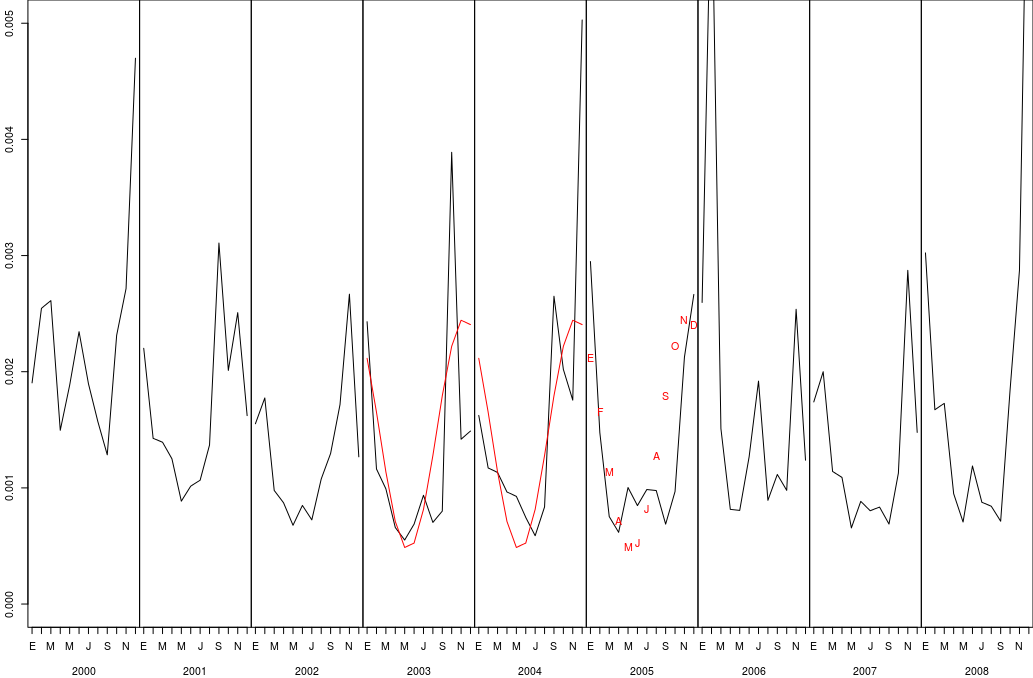
\includegraphics[scale=0.4]{img/plot_CA_2003-2005.png}
	\caption{Diverted arrivals - California}
  \end{center}
\end{figure}

Para aproximar a la funci\'on observamos algunas cosas:
\begin{itemize}  
\item Hay cierta periodicidad en la funci\'on. Posee picos en los meses correspondientes a las vacaciones de verano del hemisferio norte y descensos en el resto. El per\'iodo es de 12 meses.
\item Aunque la funci\'on tiene picos marcados, su forma se asemeja a la de $sin$ y $cos$.
\end{itemize}

Dados estos indicios nos proponemos encontrar una familia de funciones para aproximar nuestro gr\'afico usando cuadrados m\'inimos. Estas funciones ser\'an una combinaci\'on de $sin$ y $cos$ con per\'iodo 12. Las siguientes 2 familias de funciones responden a estas caracter\'isticas y aproximan relativamente bien a nuestra funci\'on, dados $alpha_i$ correspondientes.


$F_1 = \alpha_1 * abs(sin(\frac{\pi}{12}*x) * cos(\frac{\pi}{6}*x)^2) + \alpha_2$

$F_2 = \alpha_1 * sin(\frac{\pi}{6}*x) + \alpha_2 * cos(\frac{\pi}{6}*x) + \alpha_3$


La primera multiplica al $sin$ y $cos$ y toma el valor absoluto para eliminar los picos negativos. La segunda realiza la suma de los $sin$ y $cos$. No es relevante ac\'a tomar el valor absoluto ya que no hay picos marcados negativos. Luego a ambas funciones le sumamos una constante para que la curva se desplace en direcci\'on vertical. Observamos que sumar una variable lineal no ten\'ia impacto apreciable en la aproximaci\'on. 

Luego resolvimos cuadrados m\'inimos para ambas funciones y calculamos el error cuadr\'atico medio de cada una. Como training tomamos a los años 2003 y 2004 e intentamos predecir 2005.

Los errores cuadr\'aticos medios son: $ECM(F_1) = 0.0003236866$ y $ECM(F_2) = 0.0002451076$, siendo la segunda funci\'on una mejor aproximaci\'on que la primera. Los valores son pequeños ya que las mediciones son sobre un porcentaje pequeño.

Por lo tanto se puede ver en el gr\'afico anterior la aproximaci\'on que $F_2$ realiza en la muestra, prediciendo c\'omo ser\'a 2005. Se ve que respeta el comportamiento general y aproxima el pico que hay a principio y fin de año.

\subsubsection{Florida}

Realizamos el mismo an\'alisis para los vuelos dirigidos a Florida. Tomamos los mismos 
La funci\'on sigue teniendo un comportamiento peri\'odico año a año, pero en este caso vemos que por alg\'un motivo hay un desplazamiento horizontal de la curva: los picos positivos se encuentran a mitad de año.
Por otro lado, el porcentaje de vuelos desviados est\'a en el mismo rango que en California.
Dado este conjunto de similitudes y diferencias con el caso anterior, nos interes\'o ver c\'omo se comportaban nuestras familias de funciones anteriores para aproximar a nuestra nueva curva.

Para esto realizamos cuadrados m\'inimos con las siguientes dos familias de funciones:

$F_1 = \alpha_1 * abs(sin(\frac{\pi}{12}*x) * cos(\frac{\pi}{6}*x)^2) + \alpha_2$

$F_2 = \alpha_1 * sin(\frac{\pi}{6}*x) + \alpha_2 * cos(\frac{\pi}{6}*x) + \alpha_3$

y vimos que los errores cuadr\'aticos medios en este caso fueron de $ECM(F_1) = 0.0003098236$ y $ECM(F_2) = 0.0003590168$, o sea, bastante similares al anterior.

Se puede observar la curva en el siguiente gr\'afico:

\begin{figure}[h!]
  \begin{center}
	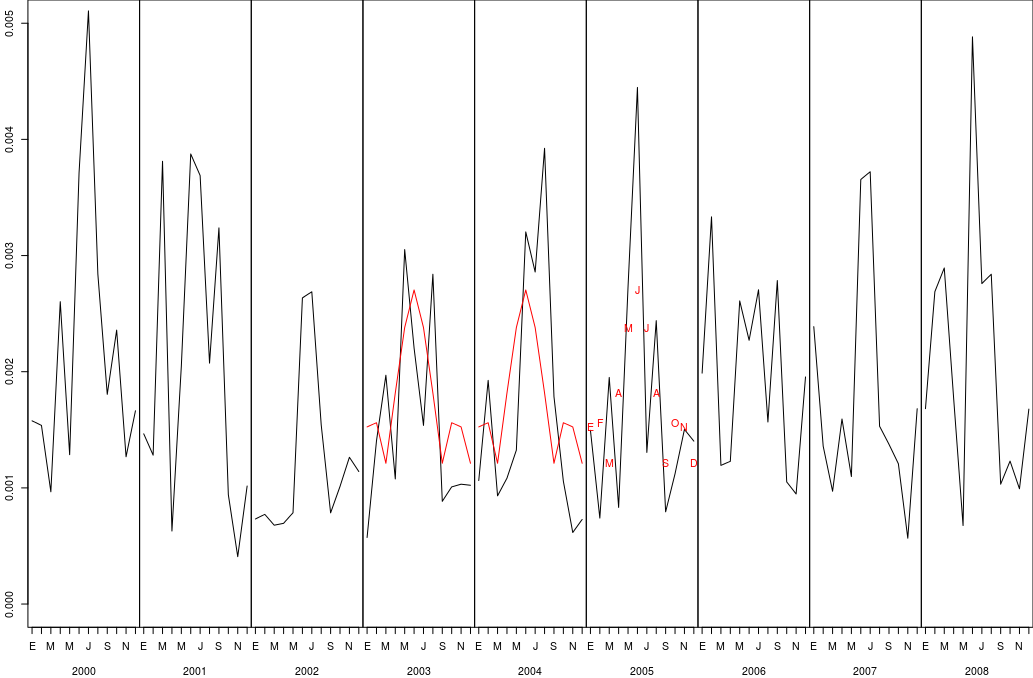
\includegraphics[scale=0.4]{img/plot_FL_2003-2005.png}
	\caption{Diverted arrivals - Florida}
  \end{center}
\end{figure}

Pero como se ve, los picos del medio son muy pronunciados, entonces quisimos crear una familia de funciones parecida  a las que ten\'iamos pero que considerase esa particularidad.
Probando un poco nos dimos cuenta que las potencias de $cos$ tienen un comportamiento de este estilo. Por ejemplo $5*cos(x)^{500} + 1$ tiene el siguiente gr\'afico:

\begin{figure}[h!]
  \begin{center}
	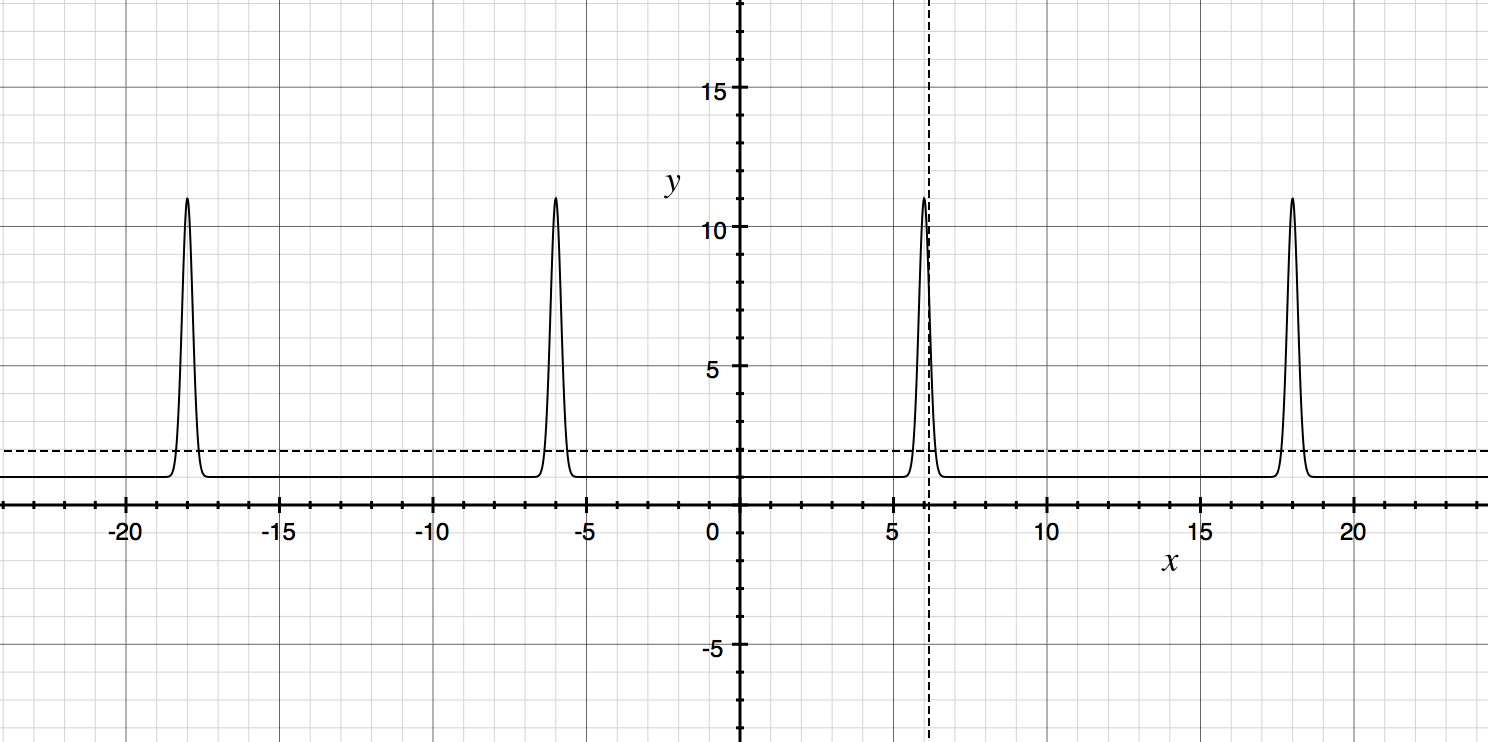
\includegraphics[scale=0.4]{img/cos500.png}
	\caption{$5*cos(x)^{500} + 1$}
  \end{center}
\end{figure}

Por lo tanto llegamos a la siguiente familia de funciones que usa esta nueva t\'ecnica.

$F_3 = \alpha_1 * abs(sin(\frac{\pi}{12}*x) * cos(\frac{\pi}{6}*x)^2) + \alpha_2 * cos(\frac{\pi}{12}*x - \frac{\pi}{2})^{500} + \alpha_3$

El error cuadr\'atico medio de esta funci\'on es $ECM(F_3) = 0.00030524$.

Podemos ver a $F_3$ representada en el gr\'afico de Florida en rojo. En ese caso se entren\'o cuadrados m\'inimos con 2003 y 2004 y se predice 2005.

\subsection{Desv\'ios por distancia}

Otro eje de análisis que nos pareció interesante fue investigar qué ocurría con la cantidad de vuelos que se desvían en relación a la distancia del viaje. Este eje surge de la idea de que a mayor distancia del viaje, mayor probabilidad de que surjan problemas en el trayecto, ya sean desperfectos técnicos, mal clima o situaciones impredecibles.

Para esto realizamos el siguiente gráfico que muestra el porcentaje de vuelos desviados según la distancia del vuelo. Como los vuelos tienen hasta 5 mil millas de distancia, partimos a nuestro conjunto en 10 subconjuntos (0 a 500 millas, 501 a 1000 millas, ..., 4501 a 5000 millas).

\begin{figure}[h!]
  \begin{center}
	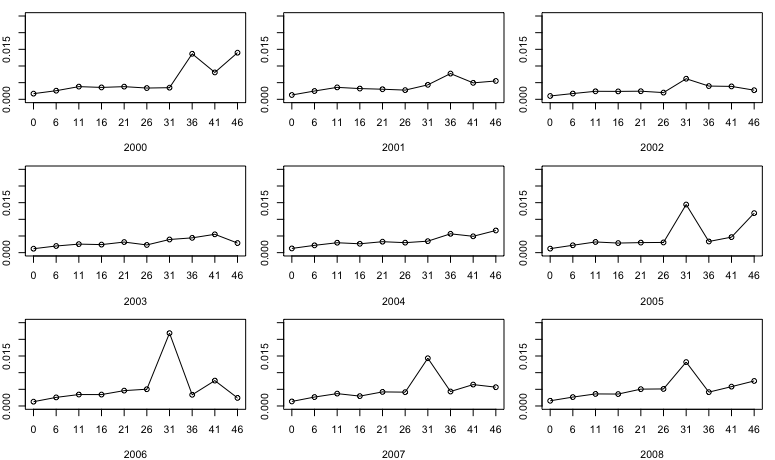
\includegraphics[scale=0.5]{img/diverted_by_distance.png}
	\caption{Diverted by distance}
  \end{center}
\end{figure}

Hay algunas cosas que se pueden ver rápidamente en el gráfico. 
Por un lado vemos que año a año la curva respeta cierto patrón. 
Por otro lado se puede ver que el gráfico acompaña la hipótesis del aumento de desvíos según la distancia del vuelo, a pesar de que la pendiente es casi nula.
La más llamativa de las características del gráfico es que en el segmento de 3001 a 3500 millas hay un pico muy llamativo, donde la cantidad de vuelos desviados llega a triplicar su valor en los segmentos aledaños. Lo más extraño es que aunque pareciera ser un outlier, este evento se da año a año, en particular entre 2005 y 2008.

Nos propusimos analizar esta situación para esclarecer sus causas. Para eso tomamos como referencia el año 2006. Primero calculamos la cantidad de vuelos que hay para cada segmento y vimos que decrece exponencialmente: mientras que para vuelos de menos de 500 millas hubo más de 3 millones, a partir de 3 mil millas los segmentos tienen menos de 5 mil vuelos. Por lo tanto los outliers tienen mucho más peso. Luego quisimos averiguar qué aeropuertos eran los que más desvíos tuvieron en el segmento del pico y los resultados son llamativos: de 47 vuelos desviados, 43 pertenecen a 2 vuelos en particular, los que vuelan entre DEN y HNL, y los que vuelan entre IAH y ANC.
Por lo tanto este pico se debe exclusivamente a características de estos 2 vuelos. Puede ser un tema climático de la ruta que utilizan, o de la administración interna de los aeropuertos con esos vuelos. Sea cual sea el motivo, es responsabilidad de muy pocos y se manifiesta en el gráfico de ese modo debido a la poca cantidad de vuelos de tanta distancia.





\section{Conclusiones}

\section{Referencias}

%\begin{thebibliography}{10}\label{bibliography}

%\bibitem{cy} Civin, P., and B. Yood, \emph{Involutions on Banach algebras}, Pacific J. Math. \textbf{9} (1959), 415--436.

%\end{thebibliography}

\end{document}